\section{Analysis of transmitting pattern}

A formal model of the transmitting pattern is fundamental for the implementation of the searching algorithm. We start from the basic Maxwell's equation and we arrive to a simpler model numerically usable.

As we will see, radiating pattern is quite complex due to the fact that we are working in the \textbf{near--field} region, condition that constraint us to not use classical DoA\marginnote{\emph{DoA}: Direction of Arrival}, such as MUSIC or ESPRIT, that operates in far-field condition and at higher frequencies. DoA systems for long waves usually requires too big electro--mechanical devices.

\subsection{Maxwell's Equations}
The following investigation is based upon Maxwell's Equation, in which the magnetic permeability $\magperm$ and dielectric constant $\dielettrico$ are considered constant (the radiation is assumed to propagate at speed of light in air). Also we consider some field properties, that are function of radio distance $\radiodist$ and time $t$:
\[
f(\radiodist,t) = f \qquad f \in \left[\; \chargedens,\; \currdens,\; \efield,\; \bfield,\; \hfield \; \right]
\]
The equations that rule the induction are the \emph{Gauss equation of magnetic induction} and the \emph{Faraday law of electric induction}:
\begin{equation}
\nabla\cdot\bfield = 0
\label{eq:gauss1}
\end{equation}
\begin{equation}
\nabla\times\efield = -\partialt \bfield
\label{eq:faraday}
\end{equation}
while the equations that rule the interaction with materials are \emph{Gauss equation} and \emph{Ampere law}:
\begin{equation}
\nabla\cdot\efield = \dfrac{\chargedens}{{\dielettrico}_0}
\label{eq:gauss2}
\end{equation}
\begin{equation}
\nabla\times\bfield = {\magperm}_0 \left( \currdens + {\dielettrico}_0 \partialt \efield \right)
\label{eq:ampere}
\end{equation}

\subsection{EM field dynamic potentials}

Starting from equation \ref{eq:gauss1}, we can define a vectorial function called \emph{potential vector} $\afield$ of $\bfield$:
\begin{equation}
\bfield = \nabla\times\afield
\label{eq:potvett}
\end{equation}
\marginnote{The existence of $\afield$ is verified by property of $\nabla$ operator, whom states that the divergence of a curl of a vector field is zero\citep{bramanti2009analisi}} 
We insert \ref{eq:potvett} in \ref{eq:faraday}:
\[
\nabla\times\efield = - \partialt \left( \nabla\times\afield \right)
\]
\begin{equation}
\nabla\times\left( \efield + \partialtarg{\afield} \right) = 0
\end{equation}
From the previous equation it is evident that the argument between parentheses is an irrotational vector field, thus a potential function exists such that:
\[
-\nabla\scpot = \efield + \partialtarg{\afield}
\]
and we derive the following definition of electric field:
\begin{equation}
\efield = - \nabla \scpot - \partialtarg{\afield}
\label{eq:efieldvett}
\end{equation}
Equation \ref{eq:potvett} and \ref{eq:efieldvett} are used to express a new formulation for the Maxwell's equation based upon vector potential\sidenote{The proof is in chapter appendix \ref{eq:evidence1}}:
\begin{equation}
\begin{array}{rcl}
\nabla^2\scpot + \partialt \nabla \cdot \afield & = & - \dfrac{\chargedens}{\dielettrico_0} \\
\nabla^2 \afield - \dfrac{1}{\velocitaluce^2} \partialttarg{\afield} - \nabla\left( \nabla \cdot \afield + \dfrac{1}{\velocitaluce^2} \partialtarg{\scpot} \right) & = & -\magperm_0 \currdens
\end{array}
\label{eq:potvecmaxwell}
\end{equation}
Those equation, even if complex, could be resolved with a well posed boundaries condition problem. Equation are coupled with the current formulation, but could be decoupled using the \textbf{Gauge transformation}\citep{mencuccini1988fisica}, also called \textbf{recalibration map}, that is in the form:
\begin{equation}
\left\{ \begin{array}{rcl}
\afield' & \mapsto & \afield + \nabla \lorentz \\
\scpot' & \mapsto & \scpot - \partialtarg{\lorentz}
\end{array}
\right.
\end{equation}
in which $\lorentz = \lorentz(\radiodist,t) \in C^2$. As proofed in \ref{eq:prooftransformationmap}, this map represents an invariant with respect to dynamic potential formulation. If we consider a $\lorentz$ such that it verifies the \textbf{Lorentz equation}
\begin{equation}
\nabla \cdot \afield' = - \dfrac{1}{\velocitaluce^2} \partialtarg{\scpot'}
\end{equation}
we obtain the decoupled version:
\begin{equation}
\begin{array}{rcl}
\nabla^2 \scpot - \dfrac{1}{\velocitaluce^2} \partialttarg{\scpot} & = & - \dfrac{\chargedens}{\dielettrico_0} \\
\nabla^2 \afield - \dfrac{1}{\velocitaluce^2} \partialttarg{\afield} & = & - \magperm_0 \currdens 
\end{array}
\end{equation}
Those dynamic equations describe the time evolution of an EM--field. If field sources are located in a finite region, the problem admit as solution a generalization of the well know stationary formulation, called retarded potential:
\begin{equation}
\begin{array}{rcl}
\scpot(\radiodist,t) & = & \dfrac{1}{4\pi \dielettrico_0} \displaystyle\iiint\limits_{\Omega} \dfrac{1}{\mid \radiodist - \radiodist' \mid} \chargedens\left( \radiodist',t-\dfrac{\mid \radiodist - \radiodist' \mid}{\velocitaluce} \right) d\radiodist   \\
\afield(\radiodist,t) & = & \dfrac{\magperm_0}{4\pi} \displaystyle\iiint\limits_{\Omega} \dfrac{1}{\mid \radiodist - \radiodist' \mid} \currdens\left( \radiodist',t-\dfrac{\mid \radiodist - \radiodist' \mid}{\velocitaluce} \right) d\radiodist 
\end{array}
\end{equation}
in which the vector distance ${\radiodist - \radiodist'}$ is the distance between the point where retarded potential is evaluated and the point where the element of volume $d\radiodist$ of the localized sources is located. The delay is due to the definition of time:
\[
t_r = t - \dfrac{\mid \radiodist - \radiodist' \mid}{c}
\]

\subsection{Magnetic dipole radiation}

\myparagraph{Potential of a magnetic dipole}
Our antenna may be seen as an ideal magnetic dipole\citep{balanis2012antenna}. The transmitting antenna is a solenoid with a ferrite core, that acts as source of the electro--magnetic field. The source is subject to a dipole magnetic moment induced by the current $J = J_0 \cos(\omegaarva t)$, with no free charges (null scalar potential). 
\begin{figure}[h]
	\centering
	
	\tdplotsetmaincoords{60}{130}
	\begin{tikzpicture}[auto,>=latex,tdplot_main_coords]
		\coordinate (origin) at (0,0,0);
		
		% Axis
		\draw [->] (origin) -- (4,0,0) node[anchor=north east]{\scriptsize{$x$}}; \draw (origin) -- (-0.2,0,0);
		\draw [->] (origin) -- (0,4,0) node[anchor=north west]{\scriptsize{$y$}}; \draw (origin) -- (0,-0.2,0);
		\draw [->] (origin) -- (0,0,2) node[anchor=south]{\scriptsize{$z$}}; \draw (origin) -- (0,0,-0.2);

		\tdplotdrawarc[->,line width=3]{(0,0,0)}{2.7}{90}{360+80}{}{}
		\tdplotdrawarc[line width=6]{(0,0,0)}{2.7}{25}{35}{}{}
		\tdplotdrawarc[<->]{(0,0,0)}{3.5}{0}{30}{anchor=north west,xshift=-10}{$\varphi'$}
		\coordinate (drpoint) at (30:2.7);
		\node at (-2.3,2.3,0) {$\mathbf{J}$};
		\node [at=(drpoint),xshift=5,yshift=-10] {$d\mathbf{r}$};

		\node [circle,draw,inner sep=1pt, fill=black] at (7.5,0,6) (rpoint) {};
		\draw[->] (origin) -- node[pos=0.8,above]{$\mathbf{r}$} (rpoint);
		\draw [dashed] (rpoint) -- (7.5,0,0) -- ++(-2.5,0,0);
		\coordinate [at=(drpoint),yshift=3] (drpoint2);
		\draw [<->] (rpoint) -- node[pos=0.425,below,xshift=-22]{$\kappa=|\mathbf{r}-\mathbf{r}'|$} (drpoint2);
		\draw [->] (origin) -- node[right]{$\mathbf{r}'$} (drpoint2);

		\tdplotsetrotatedcoords{90}{90}{180}
		\tdplotsetrotatedcoordsorigin{(origin)}
		\draw[tdplot_rotated_coords,<->] (0.5,0) arc (0:52.5:0.5) node[left,xshift=5,yshift=10]{$\theta$};

		\tdplotsetrotatedcoords{29.5+270}{-23.75}{0}
		\tdplotsetrotatedcoordsorigin{(origin)}
		\draw[tdplot_rotated_coords,<->] (0.75,0) arc (0:90:0.75) node[left,xshift=-15,yshift=10]{$\psi$};
		
	\end{tikzpicture}
	\tdplotsetmaincoords{0}{0}

	\caption{Formulation of magnetic dipole problem}
	\label{eq:dipolomagnetico}
	\forceversofloat
\end{figure}
The magnetic dipole moment is:
\begin{equation}
\magdipole = \pi r'^2\; J \vrz = m_0 \cos(\omegaarva t) \vrz
\label{eq:dipolodacorrente}
\end{equation}
From figure \ref{eq:dipolomagnetico} we define the retarded potential equation, with ${\kappa = \mid \radiodist-\radiodist'\mid}$:
\[
\afield(\radiodist,t) = \dfrac{\magperm_0}{4\pi}\int{\dfrac{J_0\cos(\omegaarva (t - \kappa/c))}{r}\ccos{\varphi'}d\varphi'}\hat{\boldsymbol{\phi}}
\]
In the hypothesis of ${\radiodist\parallel\vrz\times\vrx}$, we obtain a vector $\afield$ directed along $\vry$:
\[\begin{array}{rcl}
\radiodist & = & r \sin(\theta) \vrx + r \cos(\theta) \vrz \\
\radiodist' & = & r' \cos(\varphi') \vrx + r' \sin(\varphi') \vry \\
\kappa & = & \sqrt{(\radiodist - \radiodist')\cdot(\radiodist - \radiodist')}
\end{array}\]
Those elements in retarded potential formulation lead us to the integral formulation that has only one angular dependency:
\begin{equation}
\label{eq:integraledacalc}
\afield(\radiodist,t) = \dfrac{\magperm_0 J_0 r'}{4\pi}\int\limits_{0}^{2\pi}{\dfrac{\cos(\omegaarva (t - \kappa/c))}{\kappa} \cos(\varphi') d\varphi' \hat{\boldsymbol{\phi}}}
\end{equation}
The solution of this integral is reported in appendix; we recall only the simplification used:
\begin{itemize}
\item we assume $r' \ll r$
\item we assume $r' \ll \lambda = 2\pi c/\omegaarva$
\end{itemize}
that brings us to the following solution:
\begin{equation}
\label{eq:soluzioneint}
\afield(\radiodist,t) = \dfrac{\magperm_0 m_0}{4\pi r}\,\sin(\theta)\left( \dfrac{1}{r} \sin\left(\omegaarva(t-r/c)\right) - \dfrac{\omegaarva}{r}\cos\left(\omegaarva(t-r/c)\right)\right)\hat{\boldsymbol{\phi}}
\end{equation}
in which $m_0$ identifies the total dipole moment, considering also the number of the coils of antenna. The rest of the equation describes the propagation of the transmission in near--field conditions.

\myparagraph{Electric and magnetic field}
With null scalar potential we obtain the electric field and the magnetic field from the equations:
\begin{equation}
\begin{array}{rcl}
\efield & = & - \partialtarg{\afield} \\
\bfield & = & \nabla\times\afield 
\end{array}
\end{equation}
The application of differential operator $\nabla$:
\marginnote{In spherical coordinates: \newline $\nabla=\left[ \begin{array}{c} \dfrac{\partial}{\partial r} \\ \dfrac{1}{r}\;\dfrac{\partial}{\partial\theta} \\ \dfrac{1}{r \sin(\theta)}\;\dfrac{\partial}{\partial\phi} \end{array} \right]$}
\begin{equation}
\efield = \left[ \begin{array}{c} 0 \\ 0 \\ \partialtarg{A_{\phi}} \end{array} \right]
\qquad
\bfield = \left[ \begin{array}{c} \dfrac{1}{r}\;\dfrac{\partial A_{\phi}}{\partial \theta} \\ - \dfrac{\partial A_{\phi}}{\partial r} \\ 0 \end{array} \right]
\end{equation}
The final formulation for th EM field of a magnetic dipole is\citep{knoepfel2008magnetic}:
\begin{equation}
\begin{array}{rcl}
\label{eq:campidef1}
\tau & = &  t - \dfrac{r}{\velocitaluce} \\
E_{\phi} & = & \dfrac{\magperm_0 m_0}{4\pi}\sin(\theta)\left( \dfrac{\omegaarva}{r^2}\sin\left( \omegaarva\tau \right) + \dfrac{\omegaarva^2}{c}\cos\left( \omegaarva\tau \right) \right) \\
B_{r} & = & \dfrac{\magperm_0 m_0}{2\pi r^2}\cos(\theta)\left( \dfrac{1}{r}\cos\left( \omegaarva\tau \right) + \dfrac{\omegaarva}{c}\sin\left( \omegaarva\tau \right) \right) \\
B_{\theta} & = & \dfrac{\magperm_0 m_0}{4 \pi r^3 c^2}\sin(\theta)\left( \left( \velocitaluce^2 - \omegaarva^2 r^2 \right)\cos\left( \omegaarva\tau \right) + \omegaarva r \velocitaluce \sin\left( \omegaarva\tau \right) \right) 
\end{array}
\end{equation}
In figure \ref{fig:animazionifield} are shown some animation referred to the magnetic field defined in the previous equations. The animation are performed using ARTVA typical parameters, even if time is scaled. The equations are parametric with respect to a value, $m_0$ that is the transmitter magnetic dipole. As we have seen in chapter \ref{ch:chapter1}, the real transmitting power of an avalanche beacon is not known, but it shall have the maximum at \num{10}\si{\meter} inside a range. The animations consider an unitary magnetic dipole moment.

\begin{figure*}[p]
\label{fig:animazionifield}
\animategraphics[width=6.5cm,autoplay,loop]{15}{ch2/img/xz_10m/animation_}{0}{59}
\animategraphics[width=6.5cm,autoplay,loop]{15}{ch2/img/xz_40m/animation_}{0}{59} \newline
\animategraphics[width=6.5cm,autoplay,loop]{15}{ch2/img/xz_100m/animation_}{0}{59}
\animategraphics[width=6.5cm,autoplay,loop]{15}{ch2/img/xz_2lambda/animation_}{0}{59} \newline
\animategraphics[width=6.5cm,autoplay,loop]{15}{ch2/img/xy_10m/animation_}{0}{59} 
\animategraphics[width=6.5cm,autoplay,loop]{15}{ch2/img/xy_2lambda/animation_}{0}{59}
\caption{Graphical animation of the magnetic field $\bfield$ with retarded potential formulation. Those graph derives directly from the equations \ref{eq:campidef1}. To see the animations, please use \texttt{Adobe Acrobat viewer}}
\end{figure*}

\subsection{Magnetic field model simplification}
From animations it is evident that the effect of retarded propagation is almost null inside a radius of \num{40}\si{\meter} from the transmitting source, that is roughly the maximum distance at which an avalanche beacon receives the signal. This brings us to other simplifications for our model, as we will see in this section. From now on, all the simplifications are performed with the intent to find a model computationally convenient to be used in our algorithms.

\myparagraph{Re--definition in complex domain}
The next step is to bring equation of magnetic field in complex domain, but keeping in mind that only real part of the equations retains the physical meaning of the field. The re--interpretation is based upon Euler relationship and on the definition of wavenumber:
\[
e^{j\beta} = \ccos{\beta} + j \ssin{\beta}
\]
\[
\numeroonda = \dfrac{\omegaarva}{\velocitaluce}
\]
\begin{equation}
\begin{array}{rcl}
B_r & = & \dfrac{1}{2} \dfrac{\magperm_0 m_0}{\pi} \ccos{\theta} \braces{\dfrac{1}{r^3}\ccos{\omegaarva \tau} - \dfrac{\kappa}{r^2} \ssin{\omegaarva \tau}} \\
 & = & -\dfrac{1}{2} j \dfrac{\magperm_0 m_0}{\pi} \kappa^3 \ccos{\theta} \braces{\dfrac{1}{j^2 r^2 \kappa^2} + \dfrac{1}{j^3 r^3 \kappa^3}} e^{j\omegaarva \tau}
\end{array}
\end{equation}
\begin{equation}
\begin{array}{rcl}
B_{\theta} & = & \dfrac{1}{4} \dfrac{\magperm_0 m_0}{\pi r^3 c^2} \ssin{\theta} \braces{\braces{\velocitaluce^2 - \omegaarva^2 r^2}\ccos{\omegaarva \tau} - \omegaarva r \velocitaluce \ssin{\omegaarva \tau}} \\
 & = & -\dfrac{1}{4} j \dfrac{\magperm_0 m_0}{\pi} \kappa^3 \ssin{\theta} \braces{\dfrac{1}{j r \kappa} + \dfrac{1}{j^2 r^2 \kappa^2} + \dfrac{1}{j^3 r^3 \kappa^3}} e^{j\omegaarva \tau}
\end{array}
\end{equation}
The proof of those relations is in appendix.

\myparagraph{From Spherical to Cartesian coordinates}
\begin{marginfigure}
	\centering
	%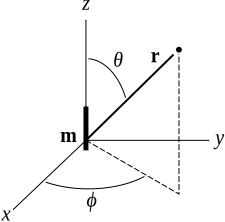
\includegraphics[width=4cm]{ch2/img/coord_pol_cart.pdf}
	\tdplotsetmaincoords{70}{110}
	\begin{tikzpicture}[auto,>=latex,tdplot_main_coords]
		\coordinate (origin) at (0,0,0);
		\tdplotsetrotatedcoords{-45}{-90}{0}
		\tdplotsetrotatedcoordsorigin{(origin)}
		%\riferimento
		% Axis
		\draw [->] (origin) -- (3,0,0) node[anchor=north east]{\scriptsize{$x$}}; \draw (origin) -- (-0.2,0,0);
		\draw [->] (origin) -- (0,2.5,0) node[anchor=west]{\scriptsize{$y$}}; \draw (origin) -- (0,-0.2,0);
		\draw [->] (origin) -- (0,0,2.5) node[anchor=south]{\scriptsize{$z$}}; \draw (origin) -- (0,0,-0.2);

		\draw[->,line width=2] (0,0,-0.1) -- node[left]{$\hat{\mathbf{m}}$} (0,0,1.5);
		\node [circle,draw,inner sep=1pt, fill=black] at (3,3,3) (rpoint) {};
		\draw [->] (origin) -- node[pos=0.8,above]{$\mathbf{r}$} (rpoint);
		\draw [dashed] (origin) -- (3,3,0) -- (3,3,3);
		\draw[tdplot_rotated_coords,<->] (2,0) arc (0:55:2) node[pos=0.5]{$\theta$};
		\draw [<->] (2,0,0) arc (0:45:2) node[pos=0.5,below]{$\phi$};
	\end{tikzpicture}
	\caption{From Sherical coordinates to Cartesian coordinates}
	\label{fig:polar2cartesian}
\end{marginfigure}
\begin{marginfigure}
	\centering
	\includegraphics[width=5cm]{ch2/img/campo_casuale.png}
	\caption{Representation of a magnetic field with source: \newline $\postx = [10, 0, 10]^T$ \newline $\magdipole=[\ccos{\pi/4},0,\ssin{\pi/4}]^T$}
	\label{fig:dipolomagneticocasuale}
\end{marginfigure}
The last approximation is related to the nature of the receiver:
\begin{itemize}
\item the receiver act as an identifier of the constant quantity of the field, or the magnitude of the oscillating field
\item the distance of the receiver is always in a radius that allows us to not consider the effect of retarded potential: 
		\[\tau = \left. t - \dfrac{r}{c} \;\right|_{r\ll c}  \longrightarrow t \]
\end{itemize}

Under those considerations, and with MacLaurin first order transformation of $B_{\theta}$, the formulation of magnetic field real part takes the form:
\begin{equation}
\bfield = \dfrac{\magperm_0}{4 \pi r^3} \braces{ 2 m_0 \ccos{\theta} \vers{r} + m_0 \ssin{\theta} \vrtheta }
\label{eq:magneticfieldpolar}
\end{equation}

The projection of the field in cartesian coordinates is:
\begin{equation}
\bfield(\radiodist,\magdipole) = \dfrac{\magperm_0}{4 \pi r^5} \magfieldmatrix \magdipole
\end{equation}
A final generalization grants us the ability to write a general form of the field that has origin in position different from the origin:
\begin{equation}
\bfield(\hexastate - \postx,\magdipole)
\end{equation}
That is the form used for our simulations.